% pyabr3 user manual (draft)
%
% Build with:  make        (from this directory; the PDF is build/pyabr3_manual.pdf)
%
% Figures: each \figorplaceholder names a file in figures/, without the extension.
% If the file is there (.png, .jpg or .pdf) it is used. If not, a box says what to
% capture. figures_needed.md lists the figures that are still needed.
%
% Text that needs information from the lab is marked with \needsinput{...}.
% Warnings about the current behaviour of the program use the caution environment;
% remove each one when that behaviour has been changed.

\documentclass[11pt,letterpaper]{report}

\usepackage[T1]{fontenc}
\usepackage[utf8]{inputenc}
\usepackage{lmodern}
\usepackage{textcomp} % \textmu (in 04_online_displays.tex) is not in T1 without it
\usepackage[margin=1in]{geometry}
\usepackage{graphicx}
\usepackage{xcolor}
\usepackage{booktabs}
\usepackage{tabularx}
\usepackage{longtable}
\usepackage{enumitem}
\usepackage{listings}
\usepackage[most]{tcolorbox}
\usepackage{tikz}
\usetikzlibrary{arrows.meta,positioning,calc,fit,backgrounds}
\usepackage{imakeidx}
\usepackage[hidelinks]{hyperref}

\graphicspath{{figures/}}
\makeindex[title=Index,intoc]

\definecolor{uncblue}{HTML}{4B9CD3}
\definecolor{needcolor}{HTML}{B3541E}
\definecolor{cautioncolor}{HTML}{A61C1C}

\setlist{itemsep=2pt,topsep=4pt}
\setlength{\parskip}{5pt}
\setlength{\parindent}{0pt}

\lstset{
  basicstyle=\ttfamily\small,
  columns=fullflexible,
  keepspaces=true,
  frame=single,
  rulecolor=\color{gray!50},
  breaklines=true,
  showstringspaces=false,
}

% names of things on the screen, and of files and keys
\newcommand{\gui}[1]{\textsf{\textbf{#1}}}
\newcommand{\file}[1]{\texttt{#1}}
\newcommand{\key}[1]{\texttt{#1}}

% information to be supplied by the lab
\newcommand{\needsinput}[1]{%
  \begin{tcolorbox}[colback=needcolor!8,colframe=needcolor,boxrule=0.5pt,arc=1pt,
                    left=4pt,right=4pt,top=2pt,bottom=2pt]
  \small\textbf{\textcolor{needcolor}{To be supplied:}} #1
  \end{tcolorbox}}

\newenvironment{caution}{%
  \begin{tcolorbox}[colback=cautioncolor!6,colframe=cautioncolor,boxrule=0.5pt,arc=1pt,
                    left=4pt,right=4pt,top=2pt,bottom=2pt]
  \small\textbf{\textcolor{cautioncolor}{Caution.}}}{\end{tcolorbox}}

% \figorplaceholder[width]{file}{caption}{what to capture}
\newcommand{\figfound}[2]{\includegraphics[width=#1,keepaspectratio]{#2}}
\newcommand{\figbox}[2]{%
  \fbox{\parbox[c][1.5in][c]{0.8\textwidth}{\centering\small
    \textbf{\textcolor{needcolor}{Figure needed:}} \texttt{figures/\detokenize{#1}}\\[4pt]#2}}}
\newcommand{\figorplaceholder}[4][0.92\textwidth]{%
  \begin{figure}[htbp]
    \centering
    \IfFileExists{figures/#2.png}{\figfound{#1}{#2.png}}{%
      \IfFileExists{figures/#2.jpg}{\figfound{#1}{#2.jpg}}{%
        \IfFileExists{figures/#2.pdf}{\figfound{#1}{#2.pdf}}{\figbox{#2}{#4}}}}
    \caption{#3}
    \label{fig:#2}
  \end{figure}}

\title{\textbf{pyabr3 User Manual}\\[6pt]
       \large Auditory brainstem response acquisition, calibration and data viewing\\[6pt]
       \large Draft for version 0.4.1}
\author{Manis Laboratory}
\date{November 2026}

\begin{document}

\pagenumbering{alph}
\maketitle
\pagenumbering{roman}
\tableofcontents
\clearpage
\pagenumbering{arabic}

\chapter{General usage and description}
\label{ch:general}

\section{What pyabr3 does}

pyabr3\index{pyabr3} records auditory brainstem responses\index{ABR}
(ABRs). It presents clicks and tone pips through a National Instruments
digital-to-analog converter and Tucker-Davis Technologies (TDT) attenuators,
records the amplified scalp potential with a TDT RP2.1 processor, and shows the
responses while the recording runs. Every repetition of every stimulus is saved in
its own file.

The program has three parts:

\begin{itemize}
  \item \textbf{Acquisition}, in the main window (Chapters~\ref{ch:acquisition}
        and~\ref{ch:online}).
  \item \textbf{Calibration} of the microphone and speaker, in its own window
        (Chapter~\ref{ch:calibration}). This replaces the calibration part of the
        MATLAB program, ABR4\index{ABR4}.
  \item \textbf{A data viewer} for recordings made by pyabr3 or ABR4
        (Chapter~\ref{ch:viewing}).
\end{itemize}

The data viewer is for checking recordings. Threshold measurement and other analysis
are done with separate code, which this manual does not cover.

\section{Example workflow}
\index{workflow}

Figure~\ref{fig:workflow} shows a typical recording day. The numbered steps in
Section~\ref{sec:example-session} follow the same order.

\begin{figure}[htbp]
\centering
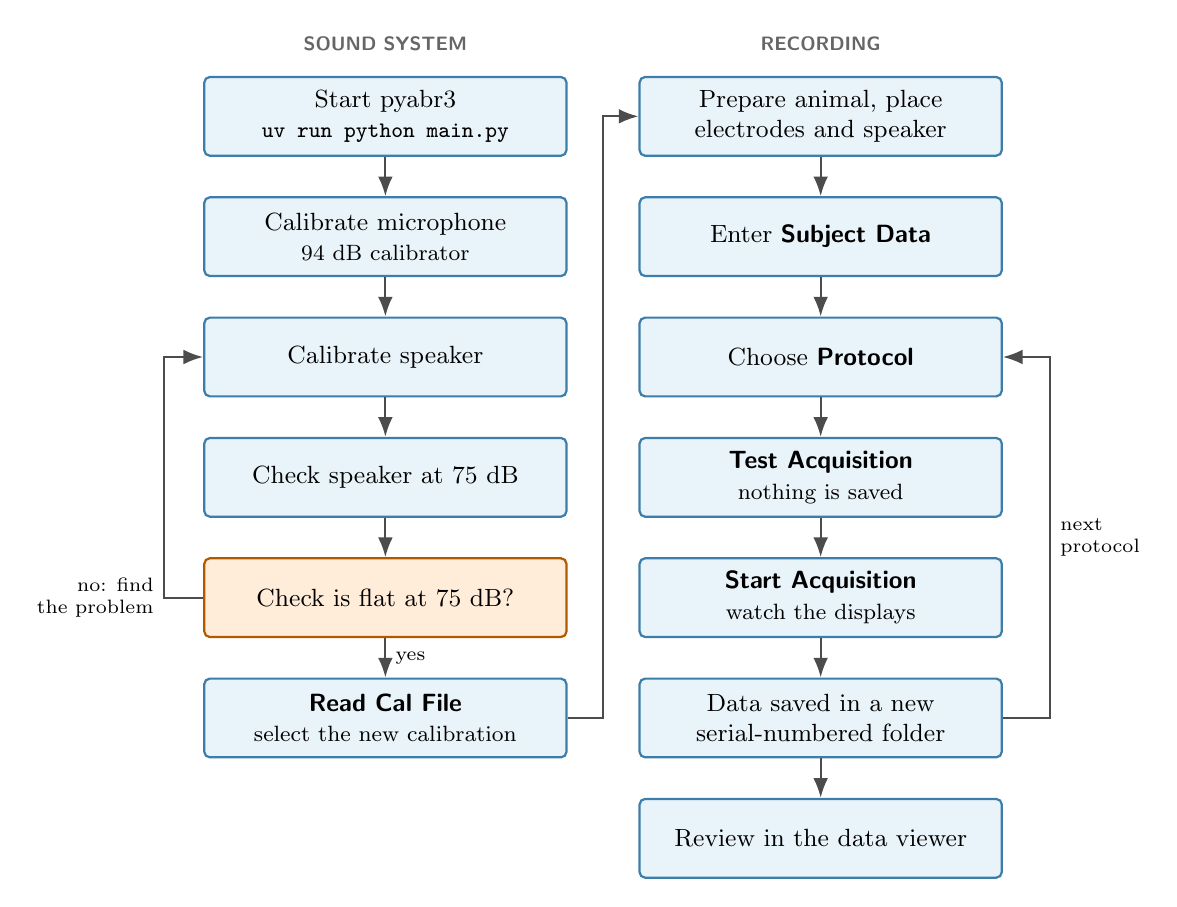
\begin{tikzpicture}[
    node distance=5mm and 9mm,
    wfbox/.style={draw=uncblue!80!black,fill=uncblue!12,rounded corners=2pt,thick,
                 minimum width=46mm,minimum height=10mm,align=center,font=\small},
    decide/.style={wfbox,fill=orange!15,draw=orange!70!black},
    flow/.style={-{Latex[length=2.5mm]},thick,draw=black!70},
    lbl/.style={font=\scriptsize\sffamily\bfseries,text=black!60}]
  % left column: preparation
  \node[wfbox] (start) {Start pyabr3\\\footnotesize\texttt{uv run python main.py}};
  \node[wfbox,below=of start] (mic) {Calibrate microphone\\\footnotesize 94~dB calibrator};
  \node[wfbox,below=of mic] (spk) {Calibrate speaker};
  \node[wfbox,below=of spk] (chk) {Check speaker at 75~dB};
  \node[decide,below=of chk] (ok) {Check is flat at 75~dB?};
  \node[wfbox,below=of ok] (read) {\gui{Read Cal File}\\\footnotesize select the new calibration};
  % right column: recording
  \node[wfbox,right=of start] (animal) {Prepare animal, place\\electrodes and speaker};
  \node[wfbox,below=of animal] (subj) {Enter \gui{Subject Data}};
  \node[wfbox,below=of subj] (proto) {Choose \gui{Protocol}};
  \node[wfbox,below=of proto] (test) {\gui{Test Acquisition}\\\footnotesize nothing is saved};
  \node[wfbox,below=of test] (run) {\gui{Start Acquisition}\\\footnotesize watch the displays};
  \node[wfbox,below=of run] (file) {Data saved in a new\\serial-numbered folder};
  \node[wfbox,below=of file] (view) {Review in the data viewer};
  % arrows
  \draw[flow] (start) -- (mic);
  \draw[flow] (mic) -- (spk);
  \draw[flow] (spk) -- (chk);
  \draw[flow] (chk) -- (ok);
  \draw[flow] (ok) -- node[right,font=\scriptsize]{yes} (read);
  \draw[flow] (ok.west) -- ++(-5mm,0) node[left,font=\scriptsize,align=right]{no: find\\the problem}
              |- (spk.west);
  \draw[flow] (read.east) -- ++(4.5mm,0) |- (animal.west);
  \draw[flow] (animal) -- (subj);
  \draw[flow] (subj) -- (proto);
  \draw[flow] (proto) -- (test);
  \draw[flow] (test) -- (run);
  \draw[flow] (run) -- (file);
  \draw[flow] (file) -- (view);
  \draw[flow] (file.east) -- ++(6mm,0) |- node[pos=0.25,right,font=\scriptsize,align=left]{next\\protocol} (proto.east);
  % headings
  \node[lbl,above=2mm of start] {SOUND SYSTEM};
  \node[lbl,above=2mm of animal] {RECORDING};
\end{tikzpicture}
\caption{A typical recording day. Calibration is not repeated for every animal; see
Section~\ref{sec:cal-overview}.}
\label{fig:workflow}
\end{figure}

\section{Where the program can run}
\index{Windows}\index{macOS}

\begin{center}
\begin{tabular}{@{}lll@{}}
\toprule
Task & Windows, with the rig hardware & macOS \\
\midrule
Acquisition & Yes & No \\
Calibration & Yes & Simulated hardware only \\
Viewing calibrations & Yes & Yes \\
Data viewer & Yes & Yes \\
\bottomrule
\end{tabular}
\end{center}

\section{Installing and starting}
\index{installation}\index{starting the program}

pyabr3 requires Python 3.13. Dependencies are managed with \file{uv}\index{uv}.
On the rig computer, the NI-DAQmx\index{NI-DAQmx} driver and the TDT drivers must
also be installed.

Run these commands from the top directory of the repository. The program finds its
configuration and protocols relative to the working directory, and will not start
from anywhere else.

\begin{lstlisting}
uv sync                       # create or update the environment
uv run python main.py         # start pyabr3
uv run python main.py test    # start with config/abrs_test.cfg
\end{lstlisting}

Without an argument, \file{main.py} uses \file{config/abrs.cfg} on Windows and
\file{config/abrs\_test.cfg} on other systems.

The calibration window and the data viewer can also be started by themselves:

\begin{lstlisting}
uv run python -m src.calibration.calibration_gui          # on the rig
uv run python -m src.calibration.calibration_gui --mock   # simulated hardware
uv run python -m src.viewer.data_viewer [file]
\end{lstlisting}

Stand-alone applications are built with \file{build\_windows.sh} and
\file{build\_macos.sh}\index{stand-alone application}.

\begin{caution}
The RP2.1 circuit is loaded from a fixed location,
\file{c:\textbackslash users\textbackslash experimenters\textbackslash desktop\textbackslash pyabr\textbackslash tdt\textbackslash abrs\_v2.rcx}.
The \key{rcx\_file} entry in the configuration file is not used. On a different
installation path, the program stops with a ``file not found'' message.
\end{caution}

\section{The main window}
\label{sec:main-window}
\index{main window}

The window has a column of parameters and controls on the left, and three tabs on the
right: \gui{Recording}, \gui{Preview} and \gui{Calibration}
(Figure~\ref{fig:main_window}). Chapter~\ref{ch:online} describes the tabs.

\figorplaceholder{main_window}{The main window before a recording, with the
\file{clickIO} protocol selected. This picture was taken on a computer with no
acquisition hardware.}{Main window at startup.}

\begin{center}
\begin{tabularx}{\textwidth}{@{}lX@{}}
\toprule
Group & Use \\
\midrule
\gui{Protocol} & Selects the protocol file. The list is read when the program starts. \\
\gui{Parameters} & Shows the values from the protocol file (see the caution below). \\
\gui{Subject Data} & Subject ID, age, sex, weight, strain, genotype and treatment group.
  These are saved with the data. \\
\gui{Actions} & The buttons that run the program (Table~\ref{tab:actions}). \\
\gui{Status} & Devices found, the current mode, and progress through the protocol. \\
\gui{Quit} & Stops the presentation and closes the program. \\
\bottomrule
\end{tabularx}
\end{center}

\begin{table}[htbp]
\centering
\caption{The \gui{Actions} group.}
\label{tab:actions}
\begin{tabularx}{\textwidth}{@{}lX@{}}
\toprule
Button & Action \\
\midrule
\gui{New Filename} & Has no effect on the names of saved files
  (Section~\ref{sec:data-files}). \\
\gui{Test Acquisition} & Presents the protocol and displays responses. Saves nothing. \\
\gui{Start Acquisition} & Presents the protocol, displays responses, and saves them. \\
\gui{Pause}, \gui{Resume} & Holds the presentation, and continues from the same place. \\
\gui{Stop} & Ends the presentation. It cannot be resumed. \\
\gui{Load Data File} & Opens the data viewer (Chapter~\ref{ch:viewing}). \\
\gui{Read Cal File} & Chooses the speaker calibration to use
  (Section~\ref{sec:cal-select}). \\
\gui{Calibrate} & Opens the calibration window (Chapter~\ref{ch:calibration}). \\
\bottomrule
\end{tabularx}
\end{table}

The \gui{Parameters} group\index{parameters!not editable} shows the values in the
selected protocol file and cannot be edited, so that a protocol of a given name is the
same from subject to subject. To use different values, save them as a new protocol file
(Section~\ref{sec:protocol-files}).

\gui{Start Acquisition} will not begin until a \gui{Subject ID}\index{Subject ID} has been
entered. The ID becomes part of the data folder name, so it cannot contain any of the
characters \verb+\ / : * ? " < > |+. \gui{Test Acquisition} saves nothing, and needs no
ID. Recordings made before this requirement store the word ``testing'' as their ID.

\section{Example session: a click intensity series}
\label{sec:example-session}
\index{example session}

\begin{enumerate}
  \item Turn on the hardware (Chapter~\ref{ch:wiring}) and start pyabr3. Check that
        \gui{Status}~/~\gui{Devices} lists the NI card, the RP2.1 and the PA5.
  \item If the sound system needs calibrating, follow
        Section~\ref{sec:cal-procedure}.
  \item Press \gui{Read Cal File} and select the calibration to use. Check its date
        and shape in the \gui{Calibration} tab.
  \item Prepare the animal, and place the electrodes and speaker.
  \item Fill in \gui{Subject Data}, including the \gui{Subject ID}, and choose the
        \gui{Data Path}.
  \item Select \file{click\_test.cfg} in \gui{Protocol}, and press
        \gui{Test Acquisition}. This presents 10 sweeps of clicks at 94~dB SPL. Check
        for a clean response in the \gui{Recording} tab, then press \gui{Stop}.
  \item Select \file{clickIO.cfg} and press \gui{Start Acquisition}. This protocol
        runs 17 levels from 90 to 10~dB SPL and takes about 7 minutes.
  \item The recording is complete when \gui{Status}~/~\gui{Mode} shows Finished.
  \item Open one of the files with \gui{Load Data File} to review the recording.
\end{enumerate}

\section{The configuration file}
\label{sec:config}
\index{configuration file}

The configuration files are in \file{config/}. The rig uses \file{abrs.cfg}.

\begin{center}
\begin{tabularx}{\textwidth}{@{}lXl@{}}
\toprule
Key & Meaning & Used? \\
\midrule
\key{required\_hardware} & Devices to connect: \texttt{NIDAQ}, \texttt{RP21},
  \texttt{PA5} & Yes \\
\key{NI\_device} & NI device name, from the NI-DAQmx utility & Yes \\
\key{calfile} & Speaker calibration read at startup. Its folder is also where the
  calibration window saves its files & Yes \\
\key{click\_reference\_dbspl} & SPL of a click at 0~dB attenuation (105.1) & Yes \\
\key{datapaths} & Named locations for saved recordings, one per line
  (Section~\ref{sec:data-files}). A single \key{datapath} entry also works & Yes \\
\key{rcx\_file} & RP2.1 circuit & No \\
\key{NI\_samplerate} & NI output rate & No (fixed at 500~kHz) \\
\key{RP21\_samplerate} & RP2.1 input rate & No (fixed at 24414.0625~Hz) \\
\key{soundcard\_output\_samplerate} & Sound card rate & No \\
\bottomrule
\end{tabularx}
\end{center}

\section{Protocol files}
\label{sec:protocol-files}
\index{protocol files}

Each file in \file{protocols/} with the extension \file{.cfg} is one protocol. To make
a new one, copy an existing file, edit it, and restart the program. This is
\file{clickIO.cfg}:

\begin{lstlisting}
# ABR Parameter file for click IO
# All times in seconds, freq in Hz
protocol:
    protocolname: 'clickIO'
    stimulustype: 'click'

stimuli:
    wave_duration: 1.2  # seconds
    stimulus_duration: 1e-4  # seconds
    stimulus_risefall: 5e-4  # seconds
    nstim: 40
    delay: 0.003 # seconds
    interval: 25e-3  # between clicks
    nreps: 20
    default_frequency: 4000.0
    default_spl: 80.0
    stimulus_period: 1e-2
    alternate: True
    dblist: [90.0, 85.0, 80.0, ... 15.0, 10.0]
    freqlist: []
recording:
    record_dur: 8e-3
    LPF: 3000.0
\end{lstlisting}

Chapter~\ref{ch:acquisition} explains each entry for each type of stimulus. The
\key{.toml} files in the same folder are not read by the program.

\section{Data files}
\label{sec:data-files}
\index{data files}\index{file names}

The \gui{Data Path}\index{Data Path} list holds the names in the \key{datapaths} entry
of the configuration file. A person can have several names, for example one for each
project. If there is more than one name, \gui{Start Acquisition} will not begin until
one has been chosen:

\begin{lstlisting}
datapaths:
    Reggie: "d:\\data\\reggie\\abr_data"
    Paul_projectA: "c:\\users\\experimenters\\desktop\\pyabr\\abr_data"
\end{lstlisting}

Each press of \gui{Start Acquisition} creates a new folder below the chosen location
(\file{<datapath>} below), and each repetition is written to one file in it:

\begin{lstlisting}
<datapath>/<date>-<Subject ID>_<serial>/<protocol>/<date>_<stimulus type>_<wave>_<repetition>.p
<datapath>/2024-12-10-p572_000/clickIO/2024-12-10_click_000_001.p
\end{lstlisting}

\file{<serial>} is the first number, from 000, for which that subject and day does not
already have a folder for the protocol. Different protocols on one subject therefore
share \file{\_000}, and a repeat of a protocol goes to \file{\_001}. Nothing is
overwritten.

\file{<wave>} counts from 0 and identifies the stimulus in the protocol.
\file{<repetition>} counts from 1. A file is a Python pickle\index{pickle} holding one
dictionary:

\begin{center}
\begin{tabularx}{\textwidth}{@{}lX@{}}
\toprule
Key & Contents \\
\midrule
\key{data} & The recorded trace, in volts at the amplifier output \\
\key{record\_frequency} & A/D sample rate, Hz \\
\key{subject\_data} & The \gui{Subject Data} fields \\
\key{protocol} & The protocol as used \\
\key{stimuli} & Levels, frequencies and attenuations of every stimulus. The waveforms
  themselves are not stored \\
\key{calibration} & The speaker calibration in use \\
\key{wave\_number}, \key{repetition} & Position in the protocol \\
\key{timestamp} & Time of writing \\
\bottomrule
\end{tabularx}
\end{center}

\gui{New Filename}\index{overwriting data} has no effect on where data are saved.

The folder arrangement below is the one that the analysis program \file{read\_abr.py}
expects. Recordings must be copied into it by hand before that program can use them:

\begin{lstlisting}
experiment_directory/
    CBA_M_N001_p48_NT/          # strain_sex_ID_age_...
        Clicks/   Tones/   Interleaved_plateau/
\end{lstlisting}

\needsinput{The lab's standard folder convention, once decided. Older recordings use
names chosen by each user, such as \file{2024-11-15-A/clicks}.}

\chapter{Calibration}
\label{ch:calibration}
\index{calibration}

\section{Overview}
\label{sec:cal-overview}

Stimulus levels in pyabr3 depend on a speaker calibration file. The file holds, for each
test frequency, the sound level that a full-scale (10~V) tone produces with no
attenuation. Making this file is a three-stage procedure, with an optional fourth
measurement:

\begin{enumerate}
  \item \textbf{Microphone:} measure the microphone's sensitivity using a sound level
        calibrator.
  \item \textbf{Speaker:} measure the sound level at each frequency at a fixed
        attenuator setting.
  \item \textbf{75~dB check:} use the new calibration to request 75~dB~SPL at every
        frequency, and measure what is produced.
  \item \textbf{Noise floor} (optional): record the microphone with no stimulus.
\end{enumerate}

\needsinput{How often the lab calibrates, and the criteria for accepting a calibration
(for example, how far the 75~dB check may deviate from 75~dB, and at which
frequencies).}

\begin{caution}
\textbf{Validation against MATLAB is not finished.}\index{validation}
The calibration code is a port of the ABR4 MATLAB program. Its formulas reproduce
stored MATLAB results, and it has been tested on simulated hardware. It has not yet
been run on the rig or compared with MATLAB on the same recordings. Until that
comparison has been made, compare new calibrations with recent MATLAB calibrations.
\end{caution}

\section{The calibration window}
\index{calibration window}

Press \gui{Calibrate} in the main window. During an acquisition, a message asks you to
stop it first. The window title shows which hardware is in use.

\begin{caution}
If the RP2.1 is not connected, the window uses \textbf{simulated hardware} and the title
says MOCK. Simulated results are written to a temporary folder, so they cannot replace a
real calibration.
\end{caution}

\figorplaceholder{cal_speaker}{The calibration window after a speaker calibration. This
example used the simulated hardware.}{Calibration window after a speaker run.}

The panel on the left holds the settings:

\begin{center}
\begin{tabularx}{\textwidth}{@{}lX@{}}
\toprule
Setting & Meaning \\
\midrule
\gui{Microphone} & The microphone in use (Table~\ref{tab:microphones}) \\
\gui{Speaker} & The speaker in use. Choosing one fills in the next two settings and
  \gui{Attn} (Table~\ref{tab:speakers}) \\
\gui{Frequencies (kHz)} & Test frequencies, separated by commas or spaces \\
\gui{Ref SPL (maxtones)} & Stored in the file \\
\gui{Cal directory} & Where files are read and written. Defaults to the folder of
  \key{calfile} in the configuration \\
\gui{Test calc (no save)} & For microphone runs: use a synthetic signal, and do not
  save \\
\gui{Mic preamp gain (dB)} & The gain set by hand on the microphone preamplifier \\
\gui{Speaker driver attn (dB)} & The setting on the speaker driver \\
\gui{Attn (dB)} & The programmable attenuator setting for speaker runs \\
\bottomrule
\end{tabularx}
\end{center}

\begin{table}[htbp]
\centering
\caption{Speaker settings. The other names in the list use the settings of the same
family.}
\label{tab:speakers}
\begin{tabular}{@{}llll@{}}
\toprule
Speaker & Frequencies & Attn & Ref SPL \\
\midrule
MF1 family & 41, from 1 to 87~kHz & 20~dB & 110 \\
EC1, ES1 family & 28, from 1 to 64~kHz & 0~dB & 83.9 \\
\bottomrule
\end{tabular}
\end{table}

\begin{table}[htbp]
\centering
\caption{Microphones, with the manufacturer's sensitivity. This is printed in the log so
that it can be compared with each measurement.}
\label{tab:microphones}
\begin{tabular}{@{}lll@{}}
\toprule
Microphone & Sensitivity (mV/Pa) & dB re 1 V/Pa \\
\midrule
7012\#39279 (1/2 inch) & 16.22 & $-35.8$ \\
7016\#9945 (1/4 inch) & 3.55 & $-49.0$ \\
7016\#10252 (1/4 inch) & 3.85 & $-48.3$ \\
\bottomrule
\end{tabular}
\end{table}

Before each run, a dialog lists the settings that the program cannot read from the
hardware (Figure~\ref{fig:cal_verify_dialog}). Check them at the equipment, and answer
\gui{Yes} only if they are correct. The values shown come from the panel on the left.

\figorplaceholder[0.45\textwidth]{cal_verify_dialog}{The settings check shown before a
speaker calibration.}{Settings confirmation dialog.}

\section{Calibration procedure}
\label{sec:cal-procedure}

\subsection{Microphone}
\index{microphone calibration}\index{calibrator}

\needsinput{How the microphone is seated in the calibrator, and the calibrator model.}

\begin{enumerate}
  \item Place the microphone in the calibrator. Set the calibrator to 94~dB and turn it
        on.
  \item Select the \gui{Microphone}, and check \gui{Mic preamp gain (dB)}.
  \item Press \gui{Microphone (94 dB)}, and confirm the settings.
  \item Read the \gui{Log}. Compare the measured transfer factor with the manufacturer's
        value printed above it.
\end{enumerate}

The program records 1~s with the attenuator at maximum. It finds the sensitivity from
the signal in a 940--1020~Hz band. The result is saved as
\file{microphone\_<name>.cal}.

\begin{caution}
\textbf{Use the 94~dB button.}\index{104 dB calibrator} After a calibration with
\gui{Microphone (104 dB)}, speaker levels read 10~dB too high. The log prints a warning
when this applies. This matches the MATLAB program, and will be corrected once
validation is complete.
\end{caution}

\figorplaceholder{cal_microphone}{A microphone calibration, using the simulated
hardware.}{Calibration window after a microphone run.}

\subsection{Speaker}
\index{speaker calibration}

\needsinput{Speaker and microphone placement for calibration, including the distance
between them and how this relates to the position of the animal.}

\begin{enumerate}
  \item Place the microphone at the position of the animal's ear.
  \item Select the \gui{Speaker}. Check \gui{Mic preamp gain (dB)},
        \gui{Speaker driver attn (dB)} and \gui{Attn (dB)}.
  \item Press \gui{Calibrate Speaker}, and confirm the settings.
\end{enumerate}

The run takes at least one minute for the MF1 frequency list. The four plots update
after each frequency. \gui{Stop} ends the run, and nothing is saved.

The run is refused if the preamplifier gain differs from the gain in the microphone's
calibration file. Measure the microphone again at the new gain, or restore the gain.

At each frequency the program:

\begin{enumerate}
  \item plays a 0.5~s, 10~V tone with 5~ms rise and fall times, and records 0.75~s from
        the microphone at 195~kHz;
  \item repeats the recording with the attenuator at maximum, to measure the noise
        floor;
  \item removes power supply noise with notch filters at 19.5--20.5~kHz and
        39--41~kHz\index{notch filters};
  \item measures the level in the middle half of the tone (25\% to 75\% of the tone
        duration), with a band-pass filter of $\pm$1/5 octave and with a cosinor fit.
\end{enumerate}

The level stored for use in stimuli, \key{maxdB}, is the band-pass measurement plus the
attenuator setting. It estimates the level at 0~dB attenuation. A frequency inside a
notch filter band produces a warning in the log, because the tone itself would be
removed.

\subsection{Check at 75 dB}
\index{75 dB check}

Leave the microphone and speaker in place, and press \gui{Check Speaker (75 dB)}. For
each frequency the program sets the attenuator to give 75~dB~SPL according to the new
calibration, then measures the result. A good calibration gives a flat line at 75~dB.
Frequencies where the speaker cannot reach 75~dB use 0~dB attenuation, and fall below
the line.

\figorplaceholder{cal_check}{A 75~dB check, using the simulated hardware.}{Calibration
window after a 75 dB check.}

\subsection{Noise floor}
\index{noise floor}

\gui{Noise Floor} records 15~s from the microphone with the attenuator at maximum. The
recording is saved as a text file, \file{Noise\_Measure\_<date and time>.csv}.

\section{Choosing the calibration to use}
\label{sec:cal-select}
\index{Read Cal File}

A new calibration is not used automatically. Press \gui{Read Cal File} in the main
window, and select a file (Figure~\ref{fig:cal_chooser}). The list shows the current
files and those in the \file{calibration\_history} folder, most recent first.
\gui{Browse for File...} finds files in other folders.

\figorplaceholder[0.6\textwidth]{cal_chooser}{The calibration file chooser.}{Calibration
file chooser.}

The chosen calibration is used for later stimuli and stored in the data files. If the
file cannot be read, a message appears and the current calibration remains in use.
Files in the older formats cannot be read.

The \gui{Calibration} tab shows the selected calibration
(Figure~\ref{fig:calibration_tab}). The upper plot shows the levels at the calibration
attenuation, the estimated maximum level, and the noise floor. The lower plot shows the
75~dB check. The check displayed is the first one made after the calibration on the same
day. If there is none, the title of the lower plot says so.

\figorplaceholder{calibration_tab}{The \gui{Calibration} tab, showing a stored
calibration from December 2024 and its 75~dB check.}{Calibration tab of the main
window.}

\section{Calibration files}
\index{calibration files}

All of these are written to the \gui{Cal directory}. Each \file{.cal} file is a MATLAB
file with the same layout as those written by ABR4. Each time one is written, a copy is
placed in \file{calibration\_history/}, with the date and time in its name.

\begin{center}
\begin{tabularx}{\textwidth}{@{}lX@{}}
\toprule
File & Contents \\
\midrule
\file{microphone\_<name>.cal} & Microphone sensitivity \\
\file{frequency\_<speaker>.cal} & Speaker calibration \\
\file{chk75db\_<speaker>.cal} & 75~dB check \\
\file{Noise\_Measure\_<date and time>.csv} & Noise floor recording (no history copy) \\
\bottomrule
\end{tabularx}
\end{center}

\chapter{Acquisition modes}
\label{ch:acquisition}
\index{acquisition}

\section{Running a protocol}
\label{sec:running}

\begin{center}
\begin{tabularx}{\textwidth}{@{}lX@{}}
\toprule
Button & Behaviour \\
\midrule
\gui{Test Acquisition} & Runs the \emph{complete} protocol with all of the displays.
  Nothing is saved. Use the protocols with \file{\_test} in their names for a short
  check. \\
\gui{Start Acquisition} & The same, and each repetition is saved as it is recorded. \\
\gui{Pause} & Holds after the current repetition. \\
\gui{Resume} & Continues from where the protocol was paused. \\
\gui{Stop} & Abandons the protocol. The attenuators return to maximum. Files that were
  already written remain. \\
\bottomrule
\end{tabularx}
\end{center}

\index{Test Acquisition}\index{Start Acquisition}\index{Pause}\index{Stop}

Several acquisitions can be run in one session.\index{repeated acquisitions} While a
protocol is running or paused, \gui{Test Acquisition} and \gui{Start Acquisition} are
refused with a message. Let the protocol finish, or press \gui{Stop}, before starting
the next.

\section{Stimulus types}
\index{stimulus types}

The \key{stimulustype} entry in the protocol file selects the type of stimulus.

\begin{table}[htbp]
\centering
\caption{The protocols provided, with their approximate minimum running time if allowed
to finish. The time counts only the waveforms and the pause after each one.}
\label{tab:protocols}
\begin{tabular}{@{}lllrr@{}}
\toprule
Protocol file & Type & Levels (dB SPL) & Freqs & Minutes \\
\midrule
\file{clickIO} & click & 90 to 10, 17 levels & -- & 7 \\
\file{click\_test} & click & 94 & -- & 0.1 \\
\file{tonepip} & tonepip & 0 to 90, 10 levels & 9 & 18 \\
\file{tonepip\_test} & tonepip & 75, 94 & 1 & 0.4 \\
\file{interleaved\_plateau} & interleaved\_plateau & 10 to 90, 9 levels & 7 & 6 \\
\file{interleaved\_plateau\_high} & interleaved\_plateau & 60 to 90, 4 levels & 7 & 1.3 \\
\file{interleaved\_plateau\_low} & interleaved\_plateau & 10 to 50, 5 levels & 7 & $<$0.1 \\
\file{interleaved\_plateau\_test} & interleaved\_plateau & 30, 90 & 2 & 0.1 \\
\bottomrule
\end{tabular}
\end{table}

\begin{caution}
\file{interleaved\_plateau\_low.cfg} currently has \key{nreps} set to 5. The intended
value is 512. Correct the file before using this protocol.
\end{caution}

\begin{caution}
\file{interleaved\_ramp.cfg} and \file{interleaved\_random.cfg} appear in the list, but
these stimulus types are not in current use and are disabled in the waveform code. They
may be enabled again in the future. Selecting one and starting an acquisition produces
an ``Unrecognized wavetype'' error.
\index{interleaved ramp}\index{interleaved random}
\end{caution}

\subsection{Clicks}
\index{click}

Each sweep is one waveform, \key{wave\_duration} seconds long. It holds \key{nstim}
clicks, each lasting \key{stimulus\_duration}, spaced by \key{interval}. The first starts at
\key{delay}~+~\key{interval}. If \key{alternate} is true, the clicks alternate in
polarity.

One waveform is used for all levels. The level is set only by the attenuator:

\[
\mathrm{attenuation} = \texttt{click\_reference\_dbspl} - \mathrm{requested\ level}
\]

\key{dblist} is the list of levels, in the order presented. \key{freqlist} is empty.

\subsection{Tone pips}
\index{tone pip}

These are built like clicks, with \key{nstim} pips of \key{stimulus\_duration}, shaped by
\key{stimulus\_risefall}. The frequencies are in \key{freqlist}. All levels of one
frequency are presented before the next frequency begins.

The attenuation is calculated from the calibration, with linear interpolation between
calibrated frequencies:

\[
\mathrm{attenuation} = \mathrm{maxdB}(f) - \mathrm{requested\ level}
\]

Before anything is presented, the program checks that the calibration can reach every
requested level (Section~\ref{sec:level-check}).

\subsection{Interleaved plateau}
\label{sec:interleaved}
\index{interleaved plateau}

All levels and frequencies are placed in one waveform, so that every combination is
presented in every sweep, rather than in separate sweeps as for clicks and tone pips.
\key{nreps} is therefore the number of sweeps for the whole protocol. Each pip starts \key{stimulus\_period} after the last one,
beginning at \key{delay}. Within the waveform, all of the frequencies at the first level
come first, then all of the frequencies at the second level, and so on.

Each pip is scaled in the waveform according to the calibration. The whole waveform is
then scaled to 10~V at its largest pip, and one attenuator setting applies to the whole
sweep. The dynamic range of the output therefore limits the range of levels that can be
combined in a protocol.

\begin{caution}
\textbf{Recordings with several interleaved sets.} Recordings that store more than one
waveform set, such as those from December 2024, repeated \key{nreps} sweeps once for each
set until stopped. The code at the time probably played them at levels below those
requested, by the smallest attenuation stored in the file (about 2.9~dB for those
recordings).
\end{caution}

The entries in the protocol file are used differently for this type:

\begin{itemize}
  \item \key{stimulus\_period} is the spacing of the pips.
  \item \key{dblist} and \key{freqlist} are text, and may contain an expression such as
        \texttt{"np.linspace(10.0, 90.0, 9)"}.
  \item \key{wave\_duration}, \key{nstim} and \key{interval} are not used. The waveform
        lasts as long as the pips require.
  \item \key{alternate} has no effect: every sweep has the same polarity.
\end{itemize}

\section{Levels that cannot be reached}
\label{sec:level-check}
\index{Cannot reach}\index{negative attenuation}

A level above the maximum for its frequency would need a negative attenuation. For
tone pips and interleaved protocols the maximum comes from the calibration in use. The
maximum for clicks is the entry \key{click\_reference\_dbspl} in the configuration
file. When \gui{Test Acquisition} or
\gui{Start Acquisition} is pressed, the program checks every level in the protocol. If
any cannot be reached, a ``Cannot reach'' message lists them with the maximum for each
frequency, nothing is presented and no folder is created. Reduce the maximum level or
the range, and save the result as a new protocol.

\section{Protocol entries}
\label{sec:protocol-entries}
\index{protocol entries}

\begin{center}
\begin{tabularx}{\textwidth}{@{}lX@{}}
\toprule
Entry & Meaning \\
\midrule
\key{stimulustype} & \texttt{click}, \texttt{tonepip} or \texttt{interleaved\_plateau} \\
\key{wave\_duration} & Duration of one sweep, s (click and tone pip only) \\
\key{stimulus\_duration} & Duration of each click or pip, s \\
\key{stimulus\_risefall} & Rise and fall time of pips, s \\
\key{nstim} & Stimuli per sweep (click and tone pip only) \\
\key{delay} & Delay added to the stimulus start times, s \\
\key{interval} & Spacing of stimuli within a sweep, s (click and tone pip only) \\
\key{nreps} & Sweeps for each stimulus. For interleaved protocols, sweeps for the whole
  protocol \\
\key{stimulus\_period} & Pause after each sweep, s. For interleaved protocols it is also
  the spacing of the pips \\
\key{alternate} & Alternate the polarity within a sweep (click and tone pip only) \\
\key{freqlist} & Frequencies, Hz \\
\key{dblist} & Levels, dB SPL \\
\key{default\_frequency}, \key{default\_spl} & Used only if the lists are absent \\
\key{record\_dur}, \key{LPF} & Saved with the data, but have no effect on acquisition \\
\bottomrule
\end{tabularx}
\end{center}

\section{Recording}
\index{recording length}\index{sample rate}

The RP2.1 records at 24414.0625~Hz. The length of a record is that of the waveform,
rounded up to a whole multiple of 1024 samples. Nothing is filtered during acquisition,
beyond any filtering in the amplifier. Filtering for display is applied when viewing
(Chapter~\ref{ch:viewing}).

\subsection{The record must fit in the buffer of the circuit}
\label{sec:record-buffer}
\index{buffer}\index{SerStore}\index{recording does not fit}\index{wave\_duration}

The ABR is stored in the buffer \texttt{sampled\_wave} of the RP2.1 circuit, a SerStore
component. \emph{The size of this buffer is fixed when the circuit is designed.} It is
the \emph{Size} of the SerStore in RPvdsEx, in 32-bit words, and the program cannot make it
larger. (The program writes the number of samples to the tag \texttt{sampled\_wave\_n},
which is connected to the Size input in the circuit, but the memory of the buffer is
allocated when the circuit is built. The program therefore uses the size compiled into
the circuit, which it reads from the circuit.) A record that is longer than the buffer
cannot be stored. When this happened on the rig (a 1.2~s record, 29696 samples, with a
buffer of 26624 samples), the data from 1090.55~ms to the end of the record repeated the
beginning of the buffer: the length was right, but the data were not valid.

\paragraph{The check.} When \gui{Test Acquisition} or \gui{Start Acquisition} is pressed,
the program works out the record needed for the longest waveform in the protocol and
compares it with the size of the buffer, read from the circuit. If it does not fit, a
message ``The recording does not fit in the buffer of the RP2.1 circuit'' gives the
sizes and what to change, nothing is presented, and no folder is created. The same check
is made again when each sweep is armed.

\paragraph{The calculation.}
\begin{enumerate}
\item Samples $=$ waveform duration $\times$ sample rate (24414.0625~Hz), rounded up to a
  whole number.
\item Rounded up to a whole multiple of 1024. This is the record, and the number of
  samples the program asks for.
\item The record must be no more than the size of the buffer.
\end{enumerate}
The longest waveform that fits is therefore
$\lfloor \mathrm{size}/1024 \rfloor \times 1024 / \mathrm{sample\ rate}$.

\begin{center}
\begin{tabular}{@{}rrrr@{}}
\toprule
Waveform (s) & Samples & Record (samples) & Record (s) \\
\midrule
0.645 (interleaved plateau) & 15748 & 16384 $= 16 \times 1024$ & 0.671 \\
1.05 & 25635 & 26624 $= 26 \times 1024$ & 1.0905 \\
1.2 (clicks and tone pips as supplied) & 29297 & 29696 $= 29 \times 1024$ & 1.2163 \\
2 & 48829 & 49152 $= 48 \times 1024$ & 2.0133 \\
5 & 122071 & 122880 $= 120 \times 1024$ & 5.0332 \\
10 & 244141 & 244736 $= 239 \times 1024$ & 10.0244 \\
\bottomrule
\end{tabular}
\end{center}

\begin{center}
\begin{tabular}{@{}rrrr@{}}
\toprule
Buffer (samples) & 24414.0625~Hz & 48828.125~Hz & 97656.25~Hz \\
\midrule
26624 & 1.0905~s & 0.5453~s & 0.2726~s \\
256000 & 10.4858~s & 5.2429~s & 2.6214~s \\
\bottomrule
\end{tabular}
\end{center}
The second table is the longest waveform that fits, for the two sizes that the circuit has
had. It shows that doubling the sample rate halves the longest record. The ABR is recorded
at 24414.0625~Hz (set in \texttt{setup\_RP21} in \file{pystim3.py}).

\paragraph{When the record is too long.} There are two cures.
\begin{itemize}
\item Make the protocol's \key{wave\_duration} short enough, using the calculation
  above. A protocol whose last stimulus ends at 1~s needs a waveform of a little more
  than that, not 1.2~s.
\item Make the buffer larger in the circuit. Open the circuit file that is loaded
  (\file{abrs\_v3.rcx} in \file{tdt\_circuits}, named in \texttt{find\_hardware} in
  \file{pystim3.py}) in RPvdsEx, and set the \emph{Size} of the SerStore that holds
  \texttt{sampled\_wave} to at least the record that is needed, in samples. For one
  channel stored as 32-bit floating point numbers, a word is a sample, and takes 4
  bytes. For example, a Size of 256000 is 1,024,000 bytes (about 1~MB), and holds
  10.4858~s at 24414.0625~Hz. For a 5~s waveform the record is 122880 samples, so a Size
  of 122880 or more is needed; for a waveform at four times the sample rate, the Size
  must be four times larger for the same duration. If the SerStore holds several
  channels, or compressed data, the number of samples per channel is the number of
  words $\times$ the compression $/$ the number of channels; the program takes this into
  account when it reads the size.
\end{itemize}
The memory of the RP2.1 is limited, and the other buffers in the circuit use it as well.
RPvdsEx shows the memory use of the circuit, which must not be exceeded. After the
circuit is changed, the program reads the new size when it is next started.

\chapter{On-line displays}
\label{ch:online}
\index{on-line displays}

\section{The Recording tab}
\index{Recording tab}

The \gui{Recording} tab comes to the front when an acquisition starts
(Figure~\ref{fig:online_recording}). The plots can be zoomed and panned with the mouse
while a protocol runs, but they are reset by later updates.

\figorplaceholder{online_recording}{The \gui{Recording} tab during a recording.}{Screen
capture from the rig during a real recording, with a clear ABR in the Average panel
(for example, clickIO at 80--90 dB SPL). Include the Status group.}

\begin{center}
\begin{tabularx}{\textwidth}{@{}lX@{}}
\toprule
Panel & Contents \\
\midrule
\gui{Raw ABR Signal} & The most recent sweeps, unfiltered, each in a different color.
  Cleared after every 10 sweeps. \\
\gui{Average ABR Signal} & The running average\index{running average}. For click and tone
  pip protocols it starts again at each new stimulus, so it shows the current level and
  frequency only. For interleaved protocols it covers the whole acquisition. \\
\gui{Waveform} & The first stimulus waveform of the protocol, drawn once at the start.
  It is shifted by 750~\textmu s, the measured delay of the output circuit. \\
Lower left and right & Reserved for intensity functions and a response map. These plots
  are not implemented and stay empty. \\
\bottomrule
\end{tabularx}
\end{center}

Time on all three plots is in milliseconds.\index{axis labels} The two response plots
show microvolts at the electrodes, using the amplifier gain of 10,000. Saved data remain
in volts at the amplifier output.

\section{Status group}
\index{Status group}

\begin{center}
\begin{tabularx}{\textwidth}{@{}lX@{}}
\toprule
Field & Meaning \\
\midrule
\gui{Devices} & Hardware that was found at startup \\
\gui{Mode} & Waiting to start, Running, Paused, Finished, or No wave loaded \\
\gui{dBSPL} & The current level (click and tone pip protocols) \\
\gui{Freq (kHz)} & The current frequency (tone pip protocols) \\
\gui{Wave \#} & The current stimulus, out of the total \\
\gui{Rep \#} & The current repetition, out of \key{nreps} \\
\bottomrule
\end{tabularx}
\end{center}

At the end of a protocol, \gui{Mode} shows Finished, and the next acquisition can be
started.

\section{Other tabs}

\gui{Preview}\index{Preview tab} is empty in this version. \gui{Calibration}%
\index{Calibration tab} shows the current calibration
(Section~\ref{sec:cal-select}).

\chapter{Viewing past data}
\label{ch:viewing}
\index{data viewer}

\section{Opening files}

Press \gui{Load Data File} in the main window, or start the viewer by itself
(Section~\ref{sec:main-window}). Then use \gui{Open File} in the viewer.

\begin{center}
\begin{tabularx}{\textwidth}{@{}lX@{}}
\toprule
File type & What is opened \\
\midrule
\file{.p} & A pyabr3 recording. Opening any one trial loads the whole recording. \\
\file{.txt} & A run from the MATLAB program, ABR4. Any file of the run may be chosen. \\
\file{.pkl} & A threshold summary such as \file{all\_tone\_map\_data.pkl}, or a file of
  numeric arrays. \\
\bottomrule
\end{tabularx}
\end{center}

\begin{caution}
\textbf{One recording per folder.} All of the \file{.p} files in a folder with the same
date and stimulus type are treated as one recording. Keep each recording in its own
folder (Section~\ref{sec:data-files}).
\end{caution}

The viewer is for checking data. Its averages match those of the analysis program, but
it does not measure thresholds or wave amplitudes.

\section{pyabr3 recordings}
\index{recordings!viewing}

The window has settings on the left, the plots on the right, and an \gui{Information}
panel below (Figure~\ref{fig:viewer_clicks}). The \gui{Information} panel shows the
subject data, protocol and calibration stored with the recording.

\figorplaceholder{viewer_clicks}{A stored click recording. The upper plot shows the
average at each level. The middle plot shows one sweep of the raw
data.}{Data viewer with a click recording.}

\begin{center}
\begin{tabularx}{\textwidth}{@{}lX@{}}
\toprule
Setting & Effect \\
\midrule
\gui{High pass}, \gui{Low pass} & Filter corners in Hz; 0 turns a filter off. The
  defaults are 300 and 3000~Hz. \\
\gui{Frequency} & The tone frequency to display \\
\gui{Interleaved set} & For interleaved recordings with more than one stimulus set,
  which set to show \\
\gui{Invert} & Inverts the polarity of the display \\
\gui{Display} & Average only; average with standard deviation; or average with
  individual traces \\
\gui{Stimulus \#}, \gui{Repetition} & Selects the sweep in the \gui{Single trial} plot \\
\bottomrule
\end{tabularx}
\end{center}

The traces are filtered forward and backward with 4-pole Butterworth filters, so no
phase shift is added. The responses are then interpolated to 100~kHz, and converted to
microvolts at the electrodes assuming an amplifier gain of 10,000\index{amplifier gain}.
The first millisecond of each response precedes the stimulus. For click and tone pip
recordings, the responses to all of the stimuli in a sweep are averaged together.

\index{standard deviation}
\gui{Average with SD} shades one standard deviation around the mean
(Figure~\ref{fig:viewer_clicks_sd}). \gui{Average with individual traces} draws up to
100 traces at each level. The first use of either view calculates the single-trial
responses, which takes a short time. The status field shows the progress.

\figorplaceholder{viewer_clicks_sd}{The same recording, with the standard deviation
shown at each level.}{Data viewer showing the average with SD.}

Figure~\ref{fig:viewer_interleaved} shows an interleaved recording. The trace for each
level and frequency is taken from its own part of the sweep.

\figorplaceholder{viewer_interleaved}{An interleaved recording, showing the responses at
16~kHz.}{Data viewer with an interleaved recording.}

The \gui{Stimulus} plot normally says that the waveform is not stored, because later
versions of the program do not save it.

\section{MATLAB (ABR4) runs}
\index{ABR4!viewing runs}\index{MATLAB runs}

A run named \file{yyyymmdd-HHMM} consists of these text files:

\begin{center}
\begin{tabular}{@{}ll@{}}
\toprule
File & Contents \\
\midrule
\file{<run>-SPL.txt} & Levels \\
\file{<run>-kHz.txt} & Frequencies (tone runs only) \\
\file{<run>-p.txt}, \file{<run>-n.txt} & Click responses for each polarity \\
\file{<run>-p-<freq>.txt}, \file{<run>-n-<freq>.txt} & Tone responses for each polarity \\
\bottomrule
\end{tabular}
\end{center}

The \gui{MATLAB run} group lists all of the runs in the folder. The two polarities are
averaged, the first 25~ms are shown, and the filter defaults are 500 and 2500~Hz.
Individual traces are not stored in these files, so only averages can be shown.

\figorplaceholder{viewer_matlab}{A run from the MATLAB program.}{Data viewer with a
MATLAB ABR4 run open. No .txt runs were available in the repository when this draft was
written.}

\begin{caution}
\index{sample rate!MATLAB runs} The sample rate of a MATLAB run is not stored in its
files. \gui{Sample rate (Hz)} is set to 100~kHz, which is correct for recent recordings.
Older recordings may have used 50~kHz. A wrong value changes the time axis and the
effect of the filters.
\end{caution}

\section{Threshold summaries}
\index{thresholds!summary files}

A \file{.pkl} file containing frequencies and thresholds, as written by
\file{read\_abr.py}, is plotted as in Figure~\ref{fig:viewer_thresholds}. Each group
appears as a mean with symbols, and each subject as a faint line. Any other \file{.pkl}
file containing numeric arrays has each array plotted.

\figorplaceholder{viewer_thresholds}{A threshold summary from
\file{all\_tone\_map\_data.pkl}.}{Data viewer showing a threshold summary.}

\chapter{Hardware wiring}
\label{ch:wiring}
\index{hardware}\index{wiring}

This chapter is an outline. It records what the software requires of the hardware,
taken from the code and from the names in the TDT circuit files. The physical
connections have not been checked on the rig, and need to be written up by someone who
has access to it.

\section{Equipment}
\index{equipment}

\begin{center}
\begin{tabularx}{\textwidth}{@{}lX@{}}
\toprule
Device & Role \\
\midrule
NI 6371\index{NI 6371} & Stimulus output at 500~kHz, $\pm$10~V, 16 bits \\
TDT RP2.1\index{RP2.1} & Records the ABR and the microphone; generates the trigger \\
TDT PA5\index{PA5} & Programmable attenuator, controlled over USB \\
Speaker driver & Drives the speaker. The setting is confirmed by hand before
  calibration \\
Speaker & MF1, EC1 or ES1 family (Table~\ref{tab:speakers}) \\
Microphone and preamplifier & Used for calibration (Table~\ref{tab:microphones}) \\
Sound level calibrator & 94~dB at 1~kHz \\
Biological amplifier & Amplifies the electrode signal, with a gain of 10,000 \\
TDT RZ5D\index{RZ5D} & Not used in this configuration. It could be used for acquisition
  if some software problems were resolved, but it cannot produce the output frequency
  needed for tones above 90~kHz \\
\bottomrule
\end{tabularx}
\end{center}

\needsinput{Exact models of the NI card, speaker driver, microphone preamplifier,
calibrator and biological amplifier, with the amplifier's filter settings.}

\section{Signal paths}
\index{signal paths}

\begin{figure}[htbp]
\centering
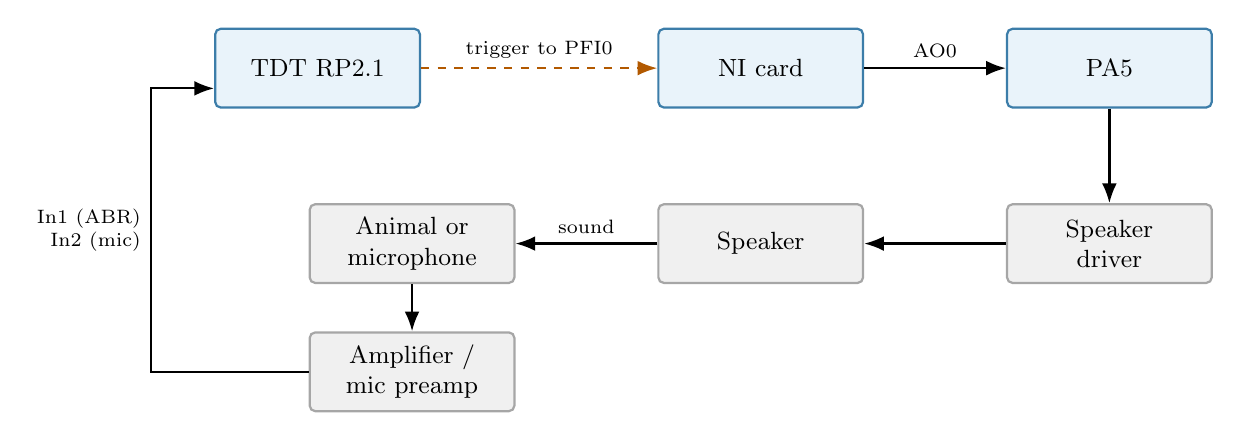
\begin{tikzpicture}[
    node distance=6mm and 10mm,
    dev/.style={draw=uncblue!80!black,fill=uncblue!12,rounded corners=2pt,thick,
                minimum width=26mm,minimum height=10mm,align=center,font=\small},
    ext/.style={dev,fill=gray!12,draw=gray!70},
    sig/.style={-{Latex[length=2.5mm]},thick},
    trg/.style={sig,dashed,draw=orange!70!black},
    pin/.style={font=\scriptsize,midway,above}]
  \node[dev] (rp) {TDT RP2.1};
  \node[dev,right=30mm of rp] (ni) {NI card};
  \node[dev,right=18mm of ni] (pa) {PA5};
  \node[ext,below=12mm of pa] (drv) {Speaker\\driver};
  \node[ext,left=18mm of drv] (spk) {Speaker};
  \node[ext,left=18mm of spk] (animal) {Animal or\\microphone};
  \node[ext,below=of animal] (amp) {Amplifier /\\mic preamp};
  \draw[trg] (rp) -- node[pin]{trigger to PFI0} (ni);
  \draw[sig] (ni) -- node[pin]{AO0} (pa);
  \draw[sig] (pa) -- (drv);
  \draw[sig] (drv) -- (spk);
  \draw[sig] (spk) -- node[pin]{sound} (animal);
  \draw[sig] (animal) -- (amp);
  \draw[sig] (amp.west) -- ++(-20mm,0) |- node[pos=0.25,left,font=\scriptsize,align=right]{In1 (ABR)\\In2 (mic)} ($(rp.south west)!0.25!(rp.north west)$);
\end{tikzpicture}
\caption{Signal paths inferred from the software. The dashed line is the trigger.}
\label{fig:signal-paths}
\end{figure}

\begin{table}[htbp]
\centering
\caption{Connections and settings that the software depends on.}
\label{tab:connections}
\begin{tabularx}{\textwidth}{@{}lXl@{}}
\toprule
Item & Requirement & Status \\
\midrule
Stimulus output & NI analog output \texttt{ao0}, $\pm$10~V & From code \\
Trigger & NI \texttt{PFI0}, rising edge, starts the stimulus. For ABR recording the
  device name in this path is fixed as \texttt{Dev1} & From code \\
Trigger source & A digital output of the RP2.1 (a BitOut block labeled ``NI Trigger Pulse
  Generator'' in both circuits) & Port to verify \\
ABR input & RP2.1 In1, stored in buffer \texttt{sampled\_wave}, at
  24414.0625~Hz & Confirmed \\
Microphone input & RP2.1 In2, read from \texttt{Data\_out2}, at
  195312.5~Hz & Confirmed \\
Attenuator & PA5 number 1, over USB. The rig has two PA5 units, but the code controls
  only this one & From code \\
RP2.1 connection & USB interface & From code \\
Amplifier gain & 10,000. The software cannot read the gain from the amplifier, so the
  data viewer uses this entered value & Confirmed \\
Mic preamp gain & 20~dB by default; must match the microphone calibration & Verify \\
Speaker driver & $-$6~dB by default & Verify \\
\bottomrule
\end{tabularx}
\end{table}

\figorplaceholder{tdt_circuit_abr}{The RP2.1 circuit used for ABR recording,
\file{tdt/abrs\_v2.rcx}.}{Export from RPvdsEx of tdt/abrs\_v2.rcx.}

\figorplaceholder{tdt_circuit_mic}{The RP2.1 circuit used for calibration,
\file{tdt/mic\_record.rcx}.}{Export from RPvdsEx of tdt/mic\_record.rcx.}

\section{Connections}

\needsinput{A cable-by-cable list: from, to, cable type and any labels. Include the
RP2.1 output that carries the trigger, which is not certain from the software.}

\figorplaceholder{hw_rack_front}{The equipment rack, front.}{Photograph of the front of
the rack, with each device labeled.}

\figorplaceholder{hw_rack_back}{The equipment rack, rear connections.}{Photograph of the
rear connections, with the trigger, output and input cables identified.}

\section{Sound delivery and recording setup}

\needsinput{Speaker position relative to the animal, free-field or closed-field use,
electrode positions and types, grounding, and steps taken to reduce electrical noise
(for example, the heating pad). Include the switch settings to be used during
recording.}

\figorplaceholder{hw_speaker_setup}{Speaker and animal position.}{Photograph of the
speaker and the animal (or a stand-in), showing distance and angle.}

\figorplaceholder{hw_electrodes}{Electrode placement.}{Photograph or drawing of the
electrode positions.}

\figorplaceholder{hw_calibrator}{The microphone in the calibrator.}{Photograph of the
microphone seated in the sound level calibrator.}

\section{Power-up and checks}
\index{power-up}

\needsinput{The order in which equipment is switched on, and a short check that the
sound path works before starting. The output stage can make noise if the attenuators
are not at maximum.}

\figorplaceholder[0.7\textwidth]{ni_max_device}{The NI device name in the NI-DAQmx
utility, as used for \key{NI\_device}.}{Screen capture of NI MAX, showing the device
name (Dev1).}


\printindex

\end{document}
